\documentclass[12pt,margin=0px]{article}

\usepackage[a4paper, margin=1in]{geometry}
\usepackage[export]{adjustbox}
\usepackage[magyar]{babel}
\usepackage[normalem]{ulem}
\usepackage[table,xcdraw]{xcolor}
\usepackage[thinlines]{easytable}
\usepackage[utf8]{inputenc}
\usepackage{amsmath}
\usepackage{amssymb}
\usepackage{amsthm}
\usepackage{enumitem}
\usepackage{fancyhdr}
\usepackage{float}
\usepackage{fontawesome}
\usepackage{geometry}
\usepackage{graphicx}
\usepackage{hhline}
\usepackage{ifthen}
\usepackage{listings}
\usepackage{makecell}
\usepackage{multirow}
\usepackage{newunicodechar}
\usepackage{pgf,tikz}
\usepackage{subcaption}
\usepackage{tipa}
\usepackage{wasysym}
\usepackage{xcolor}
\usetikzlibrary{positioning,calc,shapes.multipart,arrows,arrows.meta,matrix,automata}

\usepackage{geometry}
 \geometry{
 a4paper,
 total={170mm,297mm},
 left=20mm,
 right=20mm,
 top=20mm,
 bottom=20mm
 }

\renewcommand{\figurename}{ábra}
\newenvironment{tetel}[1]{\paragraph{#1 \\}}{}
\renewcommand{\baselinestretch}{1.15}

\newcommand{\N}{\mathbb{N}}
\newcommand{\Z}{\mathbb{Z}}
\newcommand{\R}{\mathbb{R}}
\newcommand{\Q}{\mathbb{Q}}
\newcommand{\C}{\mathbb{C}}

\definecolor{mygray}{rgb}{0.0, 0.0, 0.0}
\definecolor{blue(pigment)}{rgb}{0.2, 0.2, 0.6}
\definecolor{brickred}{rgb}{0.8, 0.25, 0.33}
\definecolor{coolblack}{rgb}{0.0, 0.18, 0.39}

\setlist[itemize,1]{label=$\bullet$}
\setlist[itemize,2]{label=$\circ$}
\setlist[itemize,3]{label=$\centerdot$}
\setlist[itemize,4]{label=$\bullet$}

% A dokument itt kezdődik
\newcommand\lword[1]{\leavevmode\nobreak\hskip0pt plus\linewidth\penalty50\hskip0pt plus-\linewidth\nobreak #1}
\date{}
\useunder{\uline}{\ul}{}
\fancyhf{} % sets both header and footer to nothing
    \lfoot{ELTE-IK}
    \cfoot{\thepage}
    \rfoot{13. tétel }

\pagestyle{fancy}

\renewcommand{\headrulewidth}{0pt}
\renewcommand{\footrulewidth}{0.4pt}

\begin{document}
    \thispagestyle{fancy}
    \hyphenation{oddword}
    \uchyph=0

    \begin{center}
        {\huge\bfseries\noindent 13. Alapvető algoritmusok és adatszerkezetek} \\
    \end{center}
    	
	\section*{Egyszerű adattípusok ábrázolásai, műveletei és fontosabb alkalmazásai}
	
    A következő öt különböző absztrakciós szintet különböztetünk meg adattípusoknál:
    \begin{enumerate}
      \item Absztrakt adattípus (ADT)
      \item Absztrakt adatszerkezet (ADS)
      \item Reprezentáció (ábrázolás)
      \item Implementáció (fejlesztés, programnyelvi megvalósítás)
      \item Fizikai (memória) szint
    \end{enumerate}

    \subsubsection*{Absztrakt adattípus (ADT)}

    \noindent Ez az adattípus leírásának legmagasabb absztrakciós szintje. Az adattípust úgy specifikáljuk ezen a szinten, hogy a szerkezetére (még) nem teszünk megfontolásokat. A leírásban kizárólag matematikai fogalmak használhatók. A specifikáció eredménye az absztrakt adattípus.\\

    \noindent Az ADT szintű specifikáció lehet formális, de lehet informális is: természetes magyar nyelven is elmondhatjuk, hogy mit várunk el például egy veremtől. A lényeg nem a leírás formalizáltsága, hanem az, hogy a specifikációban \emph{nem látjuk} az adattípus belső struktúráját.\\

    \noindent Mire jó az ADT szintű leírás?\\

    \noindent Ebben megadjuk a feladat állapotterén ($A$), illetve paraméterterén ($B$) a bemenő adatokra fennálló előfeltételeket ($Q$), majd az utófeltétel ($R$) formájában megfogalmazzuk az eredményre vonatkozó elvárásainkat. Az elő-, és utófeltétel lényegében statikus logikai állításokat tartalmaz, így a specifikáció valóban nélkülözi az algoritmikus elemeket.\\

    {\footnotesize \noindent {\color{blue} \faLightbulbO\ $\triangleright$ } }

    {\footnotesize
    \noindent Az adatszerkezetek világában is adódhatnak hasonló természetű feladatok. Amikor például egy reprezentálási mód megválasztása a kérdés, célszerű, ha úgy tudjuk leírni az adattípussal kapcsolatos elvárásainkat, hogy nem teszünk megfontolásokat a szerkezetre nézve. Ilyen például az elsőbbségi (prioritásos) sor hatékony megvalósításának a problémája. Míg a legtöbben eleve tudják, hogy milyen a verem, vagy a sor adatszerkezet, addig kevesen hozzák magukkal köznapi ismereteik részeként az elsőbbségi sor reprezentálásáról szóló tudást. Mindenképpen hasznos tehát, ha szerkezeti összefüggések nélkül definiáljuk az elsőbbségi sor fogalmát.}\\

    {\footnotesize
    \noindent Az ADT szintű leírás közvetíti az enkapszuláció gondolatát is. Ha valaki egy típust implementál, akkor az ezt tartalmazó modult várhatóan úgy írja meg, hogy magához az adatszerkezethez a felhasználó közvetlenül ne férhessen hozzá, hanem csak a műveleteken keresztül érhesse el azt. A másik oldalról, ugyanebben a szellemben, a program felhasználója is elfogadja, hogy közvetlenül nem nyúl bele egy adatszerkezetbe, hanem csak a műveletein keresztül használja és módosítja azt.}\\

    {\footnotesize
    \noindent Alapvetően két leírási mód terjedt el:
    \begin{enumerate}
        \item az algebrai specifikáció, amely logikai axiómák megadásával definiálja az absztrakt adattípust, illetve
        \item a funkcionális specifikáció, amely matematikai reprezentációval az elő-, utófeltételes módszerrel teszi ugyanezt.
    \end{enumerate}
    }
    \noindent {\footnotesize $\triangleleft$ \faLightbulbO }

    \paragraph{Algebrai specifikáció\\\\}

    \noindent Ebben a specifikációs módszerben először megadjuk az adattípus műveleteit, mint leképezéseket, az értelmezési tartományukra vonatkozó esetleges megszorításokkal együtt. Utána a műveletek egymásra hatásának értelmes összefüggéseit rögzítjük axiómák formájában.\\

    {\footnotesize \noindent {\color{blue} \faLightbulbO\ $\triangleright$ } }

    {\footnotesize
    \noindent A módszer alkalmazását a verem adattípus példáján mutatjuk be. A verem intuitív fogalma ismerős: olyan tároló struktúra, amelyből az utoljára betett elemet tudjuk kivenni. Ehhez nyilvánvalóan szerkezeti kép is társul, amelyről most tudatosan elfeledkezünk átmenetileg.\\

    \noindent Először megadjuk a verem műveleteit, mint leképezéseket. Ezek közül talán csak az Üres művelet értelmezése lehet szokatlan: egyrészt létrehoz egy vermet, amely nem tartalmaz elemeket (lásd: deklaráció a programnyelvekben), másrészt az üres verem konstans neve is. Az Üres tehát egy konstans, ezért, mint leképezés nulla-argumentumú.\\

    \noindent Az alábbi műveleteket vezetjük be:\\

    $\begin{array}{l|l|l}
        \text{Üres} & \rightarrow V & \text{Üres verem konstans; az üres verem létrehozása} \\
        \text{Üres-e} & V \rightarrow L & \text{A verem üres voltának lekérdezése} \\
        \text{Verembe} & V \times E \rightarrow V & \text{Elem betétele a verembe} \\
        \text{Veremből} & V \rightarrow V \times E & \text{Elem kivétele a veremből} \\
        \text{Felső} & V \rightarrow E & \text{A felső elem lekérdezése} \\
      \end{array}$\\\\

    \noindent Megadjuk a leképezések megszorításait. A Veremből és a Felső műveletek értelmezési tartományából ki kell vennünk az üres vermet, arra ugyanis ez a két művelet nem értelmezhető.

    $D_{\text{Veremből}}=D_{\text{Felső}}=V \backslash \{\text{Üres}\}$\\

    \noindent Az algebrai specifikáció logikai axiómák megadásával valósul meg. Sorra vesszük a lehetséges művelet-párokat és mindkét sorrendjükről megnézzük, hogy értelmes állításhoz jutunk-e.}\\
    \newpage

    {\footnotesize
    \noindent Az alábbi axiómákat írjuk fel:

    \begin{enumerate}
        \item Üres-e (Üres) vagy v=Üres $\rightarrow$ Üres-e (v)
        \item  Üres-e (v) $\rightarrow$ v=Üres
        \item  $\neg$ Üres-e (Verembe (v, e))
        \item  Veremből (Verembe (v, e))=(v, e)
        \item  Verembe (Veremből (v))=v
        \item  Felső (Verembe (v, e))=e
        \item  Felső (v)=Veremből (v).2
    \end{enumerate}

    \begin{itemize}
        \item Az 1. axióma azt fejezi ki, hogy az üres verem konstansra teljesül az üresség.\\
        Ezt változó használatával egyenlőségjelesen is megfogalmaztuk.
        \item A 2. axióma az üres verem egyértelműségét mondja ki.
        \item A 3. állítás szerint, ha a verembe beteszünk egy elemet, akkor az már nem üres.
        \item A 4-5. axiómapár mindkét sorrend esetén leírja a verembe történő elhelyezés és az elem kivétel \lword{egymásutánjának} a hatását. Mindkét esetben a kiinduló helyzetet kapjuk vissza. (Az utóbbiban a Verembe művelet argumentum-száma helyes, ugyanis a belső Veremből művelet eredménye egy (verem, elem) pár.) Az utolsó két állítás a felső elem és a vermet módosító két művelet kapcsolatát adja meg.
    \end{itemize}

    Egy ilyen axiómarendszertől először is azt várjuk, hogy helyes állításokat tartalmazzon. Természetes igény a teljesség is. Ez azt jelenti, hogy ne hiányozzon az állítások közül olyan, amely nélkül a verem meghatározása nem lenne teljes. Végül, a redundancia kérdése is felvethető: van-e olyan állítás a specifikációban, amely a többiből levezethető?\\
    }
    \noindent {\footnotesize $\triangleleft$ \faLightbulbO }

    \paragraph{Funkcionális specifikáció\\\\}

    A funkcionális specifikáció módszerében először megadjuk az adattípus matematikai reprezentációját, amelyre azután az egyes műveletek elő-, utófeltételes specifikálása épül.\\

    {\footnotesize \noindent {\color{blue} \faLightbulbO\ $\triangleright$ } }

    {\footnotesize
    A módszer a következőképp néz például sor adattípus esetén. Absztrakt szinten úgy tekinthetjük a sort, mint \emph{(elem, időpont)} rendezett párok halmazát.\\

    Az időpontok azt jelzik, hogy az egyes elemek mikor kerültek a sorba. Kikötjük, hogy az időpontok mind különbözők. Ezek után tudunk a legrégebben bekerült elemre hivatkozni.\\

    A \ref{fig:queueabs}. ábrán szereplő absztrakt sornak öt eleme van és először (legrégebben) a 40-es érték került a sorba. Ez az absztrakt reprezentáció a veremre is megfelelő lenne! A verem esetén azt az elemet választjuk ki, amelyikhez a legnagyobb időpont tartozik, a sor esetében viszont éppen a legkisebb időponttal rendelkező érték az, amely aktuálisan kivételre kerül.\\

	\begin{figure}[H]
		\centering
		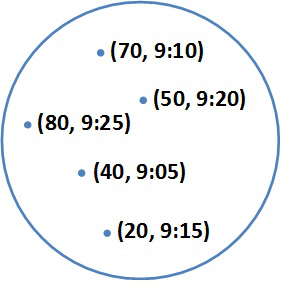
\includegraphics[width=0.3\textwidth]{img/queue_abs.png}
		\caption{A sor (és a verem) absztrakciója, mint érték-időpont párok halmaza (ADT)}
        \label{fig:queueabs}
	\end{figure}

    \noindent Formálisan ez például a következőképpen írható le (=nincs két eltérő elem azonos bekerülési idővel):
    \[
        s = \left\{ (e_i, t_i)|\ i \in \{1, \ldots, n\} \wedge n \geq 0 \wedge \forall j \in \{ 1, \ldots, n\}: i \neq j \rightarrow t_i \neq t_j \right\}
    \]

    \noindent Ha a sor műveleteit szeretnék specifikálni, akkor azt most már külön-külön egyesével is megtehetjük, nem kell az egymásra való hatásuk axiómáiban gondolkodni. Definiáljuk például a Sorból műveletet, elő-, utófeltételes specifikációval írjuk le formálisan, hogy ez a művelet a sorból az elsőkét betett elemet veszi ki, vagyis azt, amelyikhez a legkisebb időérték tartozik.

    \noindent $A = \underset{s}{S} \times \underset{e}{E}$\\
    \noindent $B = \underset{s}{S}$\\
    \noindent $Q = (s = s^{'} \wedge s^{'} \neq \emptyset)$\\
    \noindent $R = (s = s^{'}\backslash \left\{(e_{j}, t_{j}) \right\} \in \nu' \wedge e = e_{j} \wedge \forall i((e_{i}, t_{i}) \in \nu' \wedge i \neq j): t_{j} < t_{i})$\\
    }
    \noindent {\footnotesize $\triangleleft$ \faLightbulbO }

	\subsection*{Absztrakt adatszerkezet (ADS)}

    \noindent Az ADS szinten megmondjuk azt, hogy alapvetően (esetleg nem teljes részletességgel) milyen struktúrával rendelkezik a szóban forgó adattípus. Közelebbről ez azt jelenti, hogy megadjuk az adatelem közötti legfontosabb rákövetkezési kapcsolatokat, és ezt egy irányított gráf formájában le is rajzoljuk. Az absztrakt adatszerkezetet egy szerkezeti gráf és az ADT szinten bevezetett műveletek alkotják együttesen.\\

    \noindent Az ADS szinten az adattípus legfontosabb szerkezeti összefüggéseit adjuk meg egy irányított gráffal. A gráf csúcspontjai adatelemeket azonosítanak, az irányított élek pedig a közöttük fennálló rákövetkezési relációt ábrázolják.\\

    {\footnotesize \noindent {\color{blue} \faLightbulbO\ $\triangleright$ } }

    {\footnotesize
    \noindent A \ref{fig:liststack_ads}. ábrán egy nagyon egyszerű gráf látható, amely egyetlen lineáris élsorozatot tartalmaz. Ez egyaránt ábrázolhat vermet, sort vagy listát. A szövegkörnyezet dönti el, hogy melyik adattípus absztrakt szerkezetét láthatjuk az ábrán. Ha veremről van szó, akkor említésre kerül, hogy a 40-es a felső elem. Sor esetén a 40-es az első, a 80-as pedig az utolsó elem. Ha egy lista ADS szintű ábráját látjuk, akkor viszont az aktuális elem fogalmát kell szóba hozni és meg kell mondani, hogy a melyik a lista aktuális eleme; lehet az például a 20-as.}\\

    \begin{figure}[H]
		\centering
		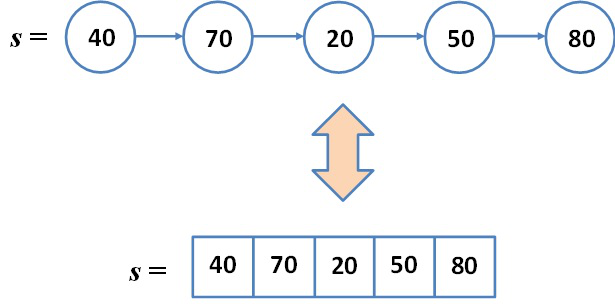
\includegraphics[width=0.6\textwidth]{img/liststack_ads.png}
		\caption{Lista (verem és sor) absztrakt szerkezeti ábrája (ADS)}
        \label{fig:liststack_ads}
	\end{figure}

    {\footnotesize
    \noindent Tegyük fel, hogy most egy absztrakt sorral van dolgunk. Az ábrán látható kétféle megjelenítés (az egzakt és az informális) megfeleltethető egymásnak. Az utóbbi a sor tömbös ábrázolása felé mutat, míg az első a láncolt ábrázolás kiindulópontjának tekinthető.\\

    \noindent Jellegzetes a bináris fa ábrája ezen a szinten, amellyel gyakran találkozhatunk. A \ref{fig:bintree_ads}. ábrán látható (gyökeres) bináris fa eredetileg irányított éleket tartalmaz, ám legtöbbször az irányítás lemarad az ábrákról. A rákövetkezéseket mutató nyilakat azonban odaértjük az élekre, szülő-gyerek irányban mindenképpen, de esetleg a fordított irányban is.\\
    }

    \begin{figure}[H]
		\centering
		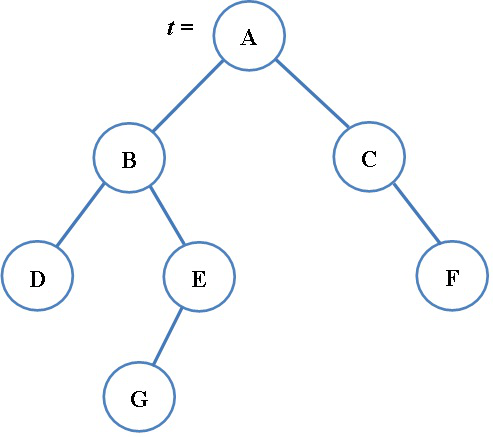
\includegraphics[width=0.45\textwidth]{img/bintree_ads.png}
		\caption{Bináris fa absztrakt szerkezeti ábrája (ADS)}
        \label{fig:bintree_ads}
	\end{figure}

    {\footnotesize
    \noindent Az ADS szint előnyeit vegyük röviden sorra.
    \begin{itemize}
        \item Ez a szint illeszkedik legjobban az ember kognitív adottságaihoz. Ennek az lehet a magyarázata, hogy éppen kellően absztrakt: már megjelenik a struktúra, de még nem kell döntést hozni az ábrázolás módjáról.
        \item A szerkezeti összefüggések lényegét emeli ki, amelyeket majd a reprezentáció szintjén teszünk teljessé.
        \item Az ADS szint szemléletes, ami nem csak a struktúrára, hanem adattípushoz tartozó műveletek illusztrálására is vonatkozik.
    \end{itemize}
    }

    \noindent {\footnotesize $\triangleleft$ \faLightbulbO }
	
    \subsection*{Adatszerkezetek reprezentálása}

    \noindent Ezen a szinten arról döntünk, hogy az ADS-szinten megjelenő gráf rákövetkezési relációit – kiegészítve azokat további szükséges szerkezeti összefüggésekkel – milyen módon ábrázoljuk. Egy adatszerkezetet többféle reprezentációval is meg lehet valósítani (pl. prioritásos sor lehet rendezetlen tömb, rendezett tömb, kupac). Két tiszta reprezentálási módot alkalmazunk.  Ezek a következők:
    \begin{itemize}
        \item Aritmetikai (tömbös) reprezentáció:  takarékos ábrázolás, elhelyezése, tetszőleges rákövetkezések, bejárások, de ezeket meg kell adni.
        \item Láncolt (pointeres) ábrázolás: minden pointer egy összetett rekord elejére mutat.
    \end{itemize}
    Az így kapott ábrázolás már az implementációhoz közeli és a számítógépes megvalósítást modellezi.

	\subsection*{Adatszerkezetek}

    \subsubsection*{Tömb}

    \begin{itemize}
        \item A tömbök legfontosabb tulajdonsága az, hogy elemei – indexeléssel – közvetlenül elérhetők. Ezt ADT szintű tulajdonságnak tekinthetjük.
        \item A tömbről ADS szinten \emph{tömbszerű} képünk van, de az elemek rákövetkezősége alapján irányított gráfként is felfoghatunk egy tömböt. Ez az absztrakció a láncolt ábrázolás felé mutat.
        \item Az megvalósítás során, az ADS szinttel összhangban, ritkán választjuk a tömb láncolt ábrázolását (ahogyan- fordítva – a listák esetében sem gyakori a tömbös megvalósítás).
        \item A tömbökről nem könnyű megmondani a felhasználás egy körében vagy konkrét esetében, hogy saját műveletekkel rendelkező önálló típusnak, vagy csupán a reprezentáció adatszerkezetének tekinthetők.
        \item A tömbök dimenziószámmal rendelkeznek; a vektor egydimenziós, míg a mátrix kétdimenziós ismert struktúra; de magasabb dimenziós tömbök használata sem ritka. A tömb erősen szemléletes fogalom; három dimenzióig könnyű elképzelni, lerajzolni a szerkezetüket.
        \item Ma már egy többdimenziós tömb, például egy mátrix nem juttatja eszünkbe, hogy a további lépésként egydimenziós tömbbel kellene reprezentálni. Ez annak köszönhető, hogy a programozási nyelvek elemi lehetőségként kínálják a többdimenziós tömbök használatát. Érdemes azonban tudatosítani, hogy többdimenziós tömbök a számítógép memóriában egydimenziósként ábrázolódnak.
        \item Speciális több dimenziós tömbök (például alsóháromszög-mátrix) helytakarékos egydimenziós ábrázolásáról olyakor magunk gondoskodunk.
    \end{itemize}

    \paragraph{A tömb absztrakt adattípus\\\\}

    \noindent Legyen $T$ az $E$ alaptípus feletti $k(\geq1)$ dimenziós tömb típus. Vezessük be az indexhalmazt $I=I_{1} \times \ldots \times I_{k}$, ahol $I_{j}=[1 \ldots n_{j}]\ (1\ \leq j\ \leq k)$.\\
    (Megjegyezzük, hogy az indexelés $1$ helyett kezdődhetne általában $m_j$-vel is, de az egyszerűség kedvéért $1$-et fogunk használni.)\\

    \noindent Az $A \in T$ tömbnek így $n=n_1 \cdot n_2 \cdot \ldots \cdot n_k$ elemet tárol, amelyek halmazát $\left\{a_1, \ldots,\ a_n \right\}$ jelöli. A $T$ tömbhöz tartozik, mint a típus meghatározó komponense, egy $f: I \rightarrow \left[1\ \ldots n\right]$ indexfüggvény, amely kölcsönösen egyértelmű leképezést létesít az indexhalmaz és az elemek halmazbeli indexei között, ezáltal egyértelmű leképzést valósít meg az indexhalmaz és a tömb elemei között. A tömbelemek egyértelműen és közvetlenül elérhetővé válnak az indexfüggvény alkalmazásával.\\

    \noindent Bevezetjük az $A[1..n_1,1..n_2,...,1..n_k]$ jelölést az A tömbre, amely magában foglalja az indexhalmazát és utal arra, hogy az indexkifejezések és a tömbelemek közötti kapcsolat is adott, így annak alapján az elemekre – indexeléssel – lehet közvetlenül hivatkozni.\\

    \noindent Bevezetjük az $A[i_1,\i _2,\ \ldots,\ i_k]$ jelölést a tömbelemek indexelésére. Ha a fenti indexfüggvény szerint $f(i_1,\ i_2,\ \ldots,\ i_k) = j$, akkor ez az indexelés az $a_j$ elemet választja ki $A[i_1,\i _2,\ \ldots,\ i_k]=a_j$. Az indexelés mechanizmusát (absztrakt megközelítésben) a \ref{fig:array_adt}. ábra szemlélteti.

	\begin{figure}[H]
		\centering
		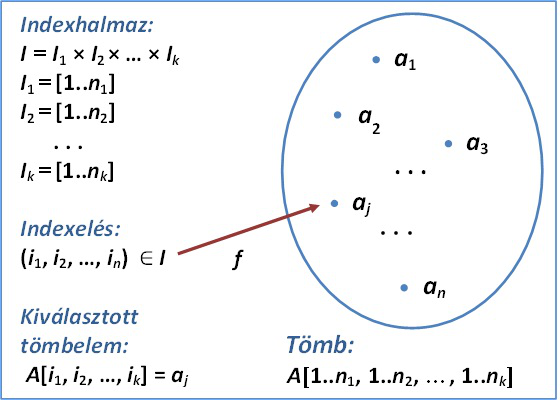
\includegraphics[width=0.5\textwidth]{img/array_adt.png}
		\caption{Tömb absztrakt adattípus}
        \label{fig:array_adt}
	\end{figure}

    \noindent A tömb műveleteinek köre szerény: a most bevezetett indexeléssel lekérdezhetjük a tömb elemeit, emellett módosíthatjuk is azokat. A tömb a mérete nem változik; nem lehet a tömbbe egy új elemet beszúrni, és nem lehet a tömbből egy elemet kitörölni. A szokás elnevezések szerint $k=1$ esetén a vektorról, $k=2$ esetén a mátrixról beszélünk.

    \paragraph{A tömb absztrakt adatszerkezet\\\\}

    \noindent A tömböktől elválaszthatatlan a szerkezetükről alkotott kép. Ezen a kép alapján például egy cellákból álló lineáris vagy négyzethálós sémában helyezzük el (az egy, illetve kétdimenziós) tömb elemeit. A \ref{fig:array_matrix_ads}. ábrán egy mátrix szokásos ábrája látható.

	\begin{figure}[H]
		\centering
		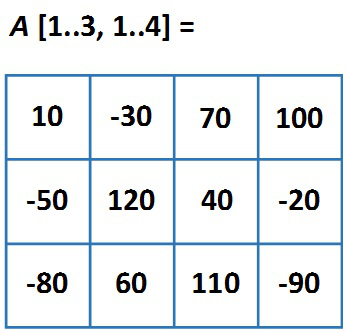
\includegraphics[width=0.35\textwidth]{img/array_matrix_ads.png}
		\caption{Tömb szemléletes képe (ADS)}
        \label{fig:array_matrix_ads}
	\end{figure}

    \noindent Az absztrakt adatszerkezet bevezetésével a fenti $f$ indexfüggvény a háttérbe húzódik, hiszen azt lehet mondani például a fenti kétdimenziós tömb esetén, hogy mondjuk az A[2,3]=40 elem a 2. sor 3. eleme, vagyis az indexkifejezést vizuálisan megjelenítettük az ADS szintű sémával.\\

    \noindent Szemléletünk számára tehát a vektor egy beosztásokkal ellátott szalag, a 2-dimenziós tömb egy mátrix, a 3-dimenziós tömb egy cellákra osztott téglatest alakját ölti gondolatainkban.\\

    \noindent Az előző, bevezető jellegű 2. fejezet szerint, az absztrakt adatszerkezetet általában egy olyan irányított gráf szemlélteti, amelyben az élek az adatelemek közötti rákövetkezéseket jelenítik meg. Egy k-dimenziós tömb elemeinek általában, a dimenziók határát kivéve, k számú rákövetkezőjük van. Formálisan is bevezethetjük a j szerinti rákövetkezés fogalmát:
    \[
        \text{köv}_{j}A\left[i_1,\ \ldots,\ i_j,\ \ldots,\ i_k\right] = A\left[i_1,\ \ldots,\ i_{j+1},\ \ldots,\ i_k\right]\quad (i_j < n_j)
    \]

    \noindent A \ref{fig:array_matrix_linked_ads}. ábra egy kétdimenziós tömb, az A[1..3,1..4] mátrix absztrakt gráfszerkezetét mutatja. Ez egy olyan ortogonális struktúra, amelyben minden csúcsból két él vezet a tömbbeli rákövetkezőkhöz.

	\begin{figure}[H]
		\centering
		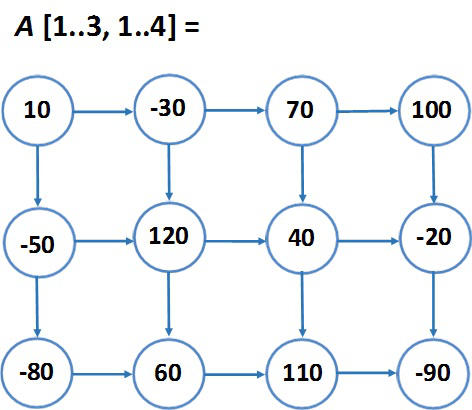
\includegraphics[width=0.4\textwidth]{img/array_matrix_linked_ads.png}
		\caption{Tömb gráfja (ADS)}
        \label{fig:array_matrix_linked_ads}
	\end{figure}

    \noindent Valójában a tömbről nem ilyen képet őrzünk fejünkben, ahogyan a verem sem egy lineáris gráf formájában rögzül a memóriánkban. Annyiban azonban mégsem fölösleges a gráfos szemlélet, mert közelebb hozza a ritka mátrixok láncolt ábrázolásának ötletét.

    \subsection*{A tömb megvalósításai}

    \paragraph{Aritmetikai reprezentáció\\\\}

    \noindent Egy adatszerkezet aritmetikai ábrázolása során az adatelemeket egy tömbben helyezzük el, az eredeti strukturális összefüggéseket pedig függvények formájában adjuk meg.\\

    \noindent Az adatokat tároló tömb lehet egy- vagy többdimenziós. Szemléletünk számára egy többdimenziós tömb már annyira egyszerű adatszerkezet, hogy nem szükséges mindig újra meggondolni az egydimenziós elhelyezés lehetőségét. A programnyelvek is megerősítenek ebben, hiszen a többdimenziós tömbök használatát az alapvető lehetőségek között nyújtják.\\

    \noindent A tömb adattípus ismertetésekor azonban, legalább ezen a helyen egyszer, érdemes szóba hozni azt, hogy a többdimenziós tömbök elemeit még el kell helyezni a szalagszerű egydimenziós memóriában.\\

    \noindent A szekvenciális tárolást általában a sorfolytonos vagy oszlopfolytonos módszerrel szokás megoldani. (Azzal még itt sem foglalkozunk, hogy a tárolás végállomása egy bájtokból álló vektor, és a bájtokat – még tovább finomítva – bitek sorozata alkotja.)\\

    \noindent A \ref{fig:array_storage_one}. ábrán a korábban is szereplő mátrixnak az egydimenziós tárolást illusztrálja, mindkét elhelyezési stratégia szerint.

	\begin{figure}[H]
		\centering
		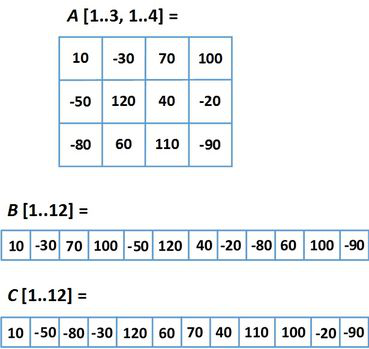
\includegraphics[width=0.4\textwidth]{img/array_storage1.png}
		\caption{Kétdimenziós tömb egydimenziós tárolása}
        \label{fig:array_storage_one}
	\end{figure}

    \noindent A kapcsolatot az elemek mátrixban elfoglalt pozíciója és az új helye között index-függvényekkel adjuk meg. Egy $A[1 \ldots m, 1\ldots n]$ kétdimenziós tömbre, például a sorfolytonos esetben ez a következő:
    \[
        ind(i,j) = (i-1)n + j
    \]

    \paragraph{Láncolt ábrázolás\\\\}

    \noindent Bizonyos (jobbára gazdasági) problémák modellezése nagyméretű mátrixok alkalmazásához vezet. Előfordul azonban, hogy a mátrix csekély értékes adatot tárol. Ilyenkor gondolhatunk arra a reprezentálási módra, amelyet a \ref{fig:array_linked_list}. ábrán láthatunk.

    \noindent A ritka mátrixok láncolt ábrázolásában csak az értékes elemek szerepelnek. Alkalmazhatunk egyirányú láncolást, amelyben minden elemtől a sor- és oszlopbeli rákövetkezőjéhez irányít a két tárolt pointer. A sorok és az oszlopok bejárataira, pontosabban az első bennük szereplő elemre, egy-egy fejelem mutat, amelyek maguk is egy-egy listát alkotnak. A két fejelem lista egy közös fejelemből érhető el.

	\begin{figure}[H]
		\centering
		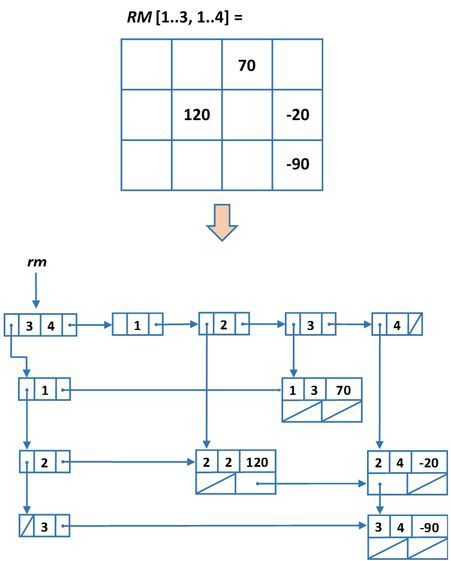
\includegraphics[width=0.4\textwidth]{img/array_linked_list.png}
		\caption{Ritka mátrix láncolt ábrázolása}
        \label{fig:array_linked_list}
	\end{figure}

    \noindent Az ábra nem csak a helytakarékosság lehetőségét érzékelteti, hanem azt is, hogy ezzel az ábrázolási móddal feladtuk az elemek közvetlen indexelhetőségét és csak meglehetős nehézkességgel tudunk eljutni az elemekhez.\\

    \noindent Az elemek elérését, illetve a struktúrában való mozgást valamelyest javítja, ha kétirányú láncolást alkalmazunk, mind a sorokban és az oszlopokban, mind pedig a két fejelem-listában.\\

    \noindent Azt a kérdést, hogy alkalmazzuk-e adott esetben ezt a tárolási formát, két szempont dönti el. Egyik a helytakarékosság kérdése: az értékes mátrixelemek (várható) számának és méretének ismerete esetén könnyen kiszámítható, hogy előnyösebb-e ez az ábrázolás, mint a hagyományos. Ehhez csak a pointerek számát kell meghatározni, amelyet a memóriacím helyfoglalásával (ami általában 2 vagy 4 bájt) szorozva kell a memóriaigény számításában figyelembe venni.\\

    \noindent A másik mérlegelendő szempont az, hogy mennyire támogatják a feldolgozó eljárások megvalósíthatóságát a láncolt adatszerkezeten való közlekedés korlátozott lehetőségei. \\
    A mai memóriakapacitások mellett lehet, hogy ez a súlyosabb szempont. Ha arra gondolunk például, hogy hogyan kellene két ritka mátrix összegét előállítani, akkor látható, hogy a láncolt ábrázolás mellett a legegyszerűbb feladat megoldása is körülményessé válhat.\\

	\begin{itemize}
		\item \textit{Tömb}: Azonos típusú elemek sorozata, fix méretű.
		\item \textit{Verem}: Mindig a verem tetejére rakjuk a következő elemet, csak a legfelsőt kérdezhetjük le, és vehetjük ki.
		\begin{figure}[H]
			\centering
			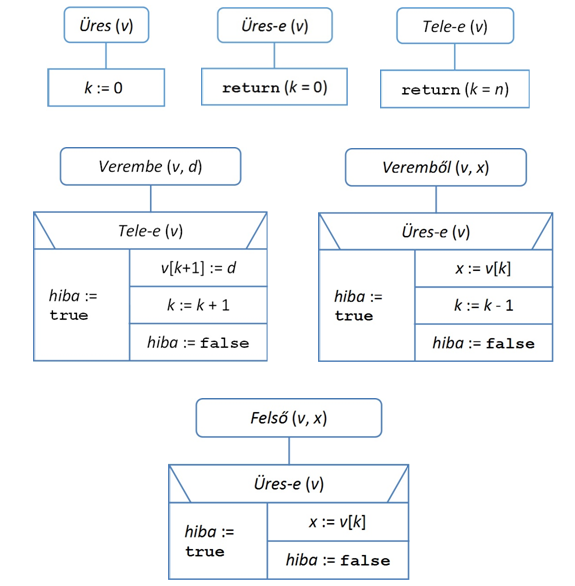
\includegraphics[width=0.6\textwidth]{img/stack_operations.png}
			\caption{Verem műveletei}
		\end{figure}
		\item \textit{Sor}: Egyszerű, elsőbbségi és kétvégű. A prioritásos sornál az elemekhez tartozik egy érték, ami alapján rendezhetjük  őket.
		\begin{figure}[H]
			\centering
			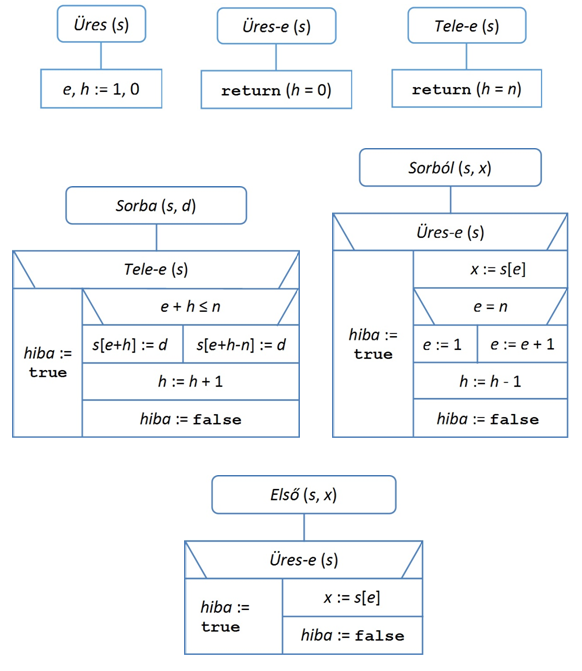
\includegraphics[width=0.6\textwidth]{img/queue_operations.png}
			\caption{Sor műveletei}
		\end{figure}
        \item \textit{Lista}: Láncolt ábrázolással reprezentáljuk. 3 szempont szerint különböztethetjük meg a listákat: fejelem van/nincs, láncolás iránya egy/kettő, ciklusosság van/nincs. Ha fejelemes a listánk, akkor a fejelem akkor is létezik, ha üres a lista.\\
        A lista node-okból áll, minden node-nak van egy, a következőre mutató pointere, illetve lehet az előzőre is, ha kétirányú. Ezen kívül van egy első és egy aktuális node-ra mutató pointer is, és az utolsó elem mutatója NIL. A listát megvalósíthatjuk úgy, hogy tetszőleges helyre lehessen elemet beszúrni, illetve törölni.

		\begin{figure}[H]
			\centering
			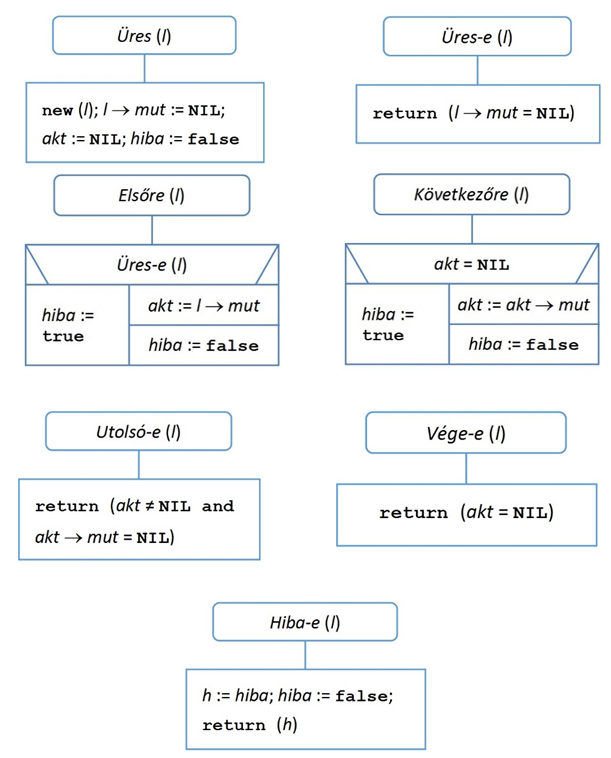
\includegraphics[width=0.55\textwidth]{img/list_operations1.png}
			\caption{Lista műveletei}
		\end{figure}

		\begin{figure}[H]
			\centering
			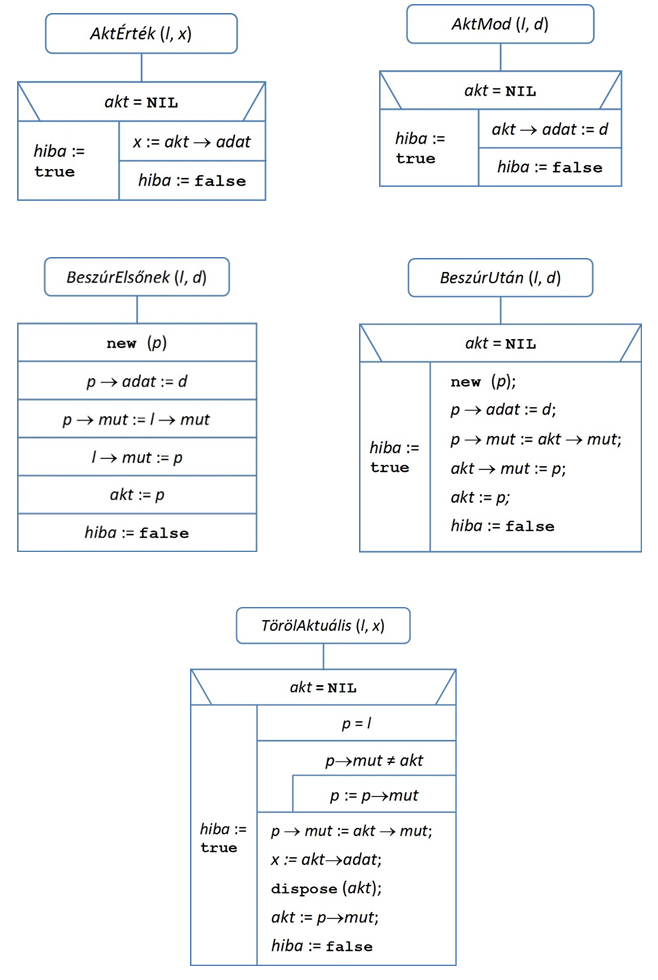
\includegraphics[width=0.55\textwidth]{img/list_operations2.png}
			\caption{Lista műveletei}
		\end{figure}

        \item \textit{Fa}: Egyszerű, bináris és speciális (kupac, bináris keresőfa, AVL-fa). A bináris fát rekurzívan definiáljuk: $t \in T(E)$ [bin. fák típusérték halmaza(alaptípus)] $t$ üres fa (jele: $\Omega$), vagy $t$-nek van gyökéreleme, $bal(t)$, $jobb(t)$ részfája. Láncoltan ábrázoljuk, tömbösen csak teljes fák, illetve kupac esetén.
        \item \textit{Kupac}: Olyan bináris fa, melynek alakja majdnem teljes és balra rendezett. Tömbösen ábrázoljuk, mert pointeresen a bonyolult lépkedést nem teszi lehetővé, tömbösen indexösszefüggésekkel könnyen megoldható.
		\begin{figure}[H]
			\centering
			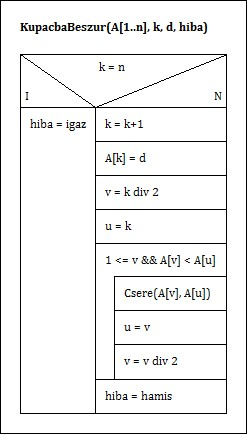
\includegraphics[width=0.3\textwidth]{img/KupacbaBeszur.jpg}
			\caption{Kupac műveletei}
		\end{figure}
		\item \textit{Hasítótábla}
		\item \textit{Gráf} [Nem egyszerű adattípus.]
	\end{itemize}
	
	\subsection*{Adatszerkezetek lehetséges műveletei}
	
	\begin{itemize}
		\item Üres adatszerkezet létrehozása
		\item Annak lekérdezése, hogy üres-e az adatszerkezet
		\item Elem berakása, itt ellenőrizni kell, hogy nem telt-e még meg
		\item Elem kivétele vagy törlése, itt ellenőrizni kell, hogy nem üres-e
		\item Adott tulajdonságú elem (például maximum, veremben a felső) lekérdezése, itt is ellenőrizni kell, hogy üres-e az adatszerkezet
		\item Bejárások (preorder, inorder, postorder, szintfolytonos), listáknál az első, előző vagy következő elemre lépés
		\item Elem módosítása bizonyos adatszerkezeteknél (pl. listák)
	\end{itemize}
	
	\subsection*{Fontosabb alkalmazásai}
	
    \textit{Prioritásos sor}: nagygépes programfuttatásnál az erőforrásokat a prioritás arányában osszuk el, adott pillanatban a maximális prioritásút válasszuk. Sürgősségi ügyeleten, gráfalgoritmusoknál is alkalmazható.
	\textit{B-fa}: ipari méretekben adatbázisokban használják.
	
	\section*{A hatékony adattárolás és visszakeresés néhány megvalósítása}
	
	\subsection*{Bináris keresőfa}
	
    \noindent A bináris keresőfa a kulcsos adatrekordok tárolásának egyik elsőként kialakult eszköze. Egyszerű tárolási elvet valósít meg: a legelső, a gyökérben elhelyezett rekord utáni kulcsokat a \emph{kisebb balra, nagyobb jobbra} elv alapján illesztjük be a fába. A kiegyensúlyozással kiegészítve a tárolás hatékony adatszerkezetét kapjuk (AVL-fa, piros-fekete fa).\\

    \noindent A bináris keresőfa nevezetes tulajdonsága az, hogy inorder bejárással a kulcsokat rendezett sorozatként érjük el. Ez következik az inorder bejárás azon tulajdonságaiból, hogy
    \begin{enumerate}
        \item a gyökeret középen, a bal oldali és a jobb oldali részfa bejárása között érintjük,
        \item a bal oldali részfa minden kulcsa kisebb, a jobb oldali minden kulcsa nagyobb, mint a gyökérben tárolt kulcs és
        \item mindkét oldali részfát inorder módon járjuk be.
    \end{enumerate}

	\begin{figure}[H]
		\centering
        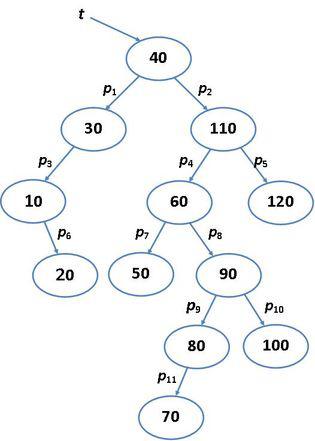
\includegraphics[width=0.26\textwidth]{img/bin_tree_sample1.png}
		\caption{Bináris keresőfa}
		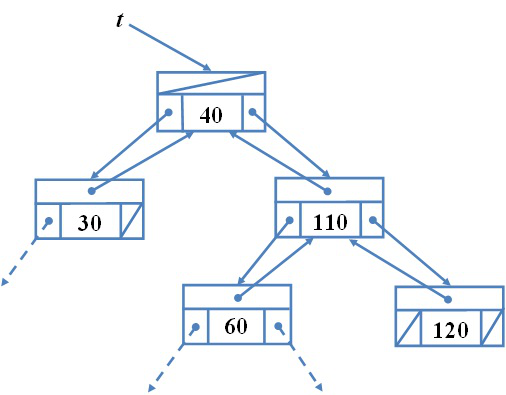
\includegraphics[width=0.4\textwidth]{img/bin_tree_sample2.png}
        \caption{Bináris keresőfa láncolt ábrázolása}
	\end{figure}

    \noindent Adjuk meg a bináris keresőfa definícióját. A felépítés dinamikus szabálya után statikus meghatározást keresünk. A $t$ bináris fát pontosan akkor mondjuk egyúttal bináris keresőfának, ha $t$ bármely $x$ csúcsára igaz az, hogy amennyiben $y$ az $x$ bal oldali részfájának egy csúcsa, illetve ha a $z$ pont az $x$ jobb oldali részfájának egy csúcsa, akkor
    \begin{center}
      $kulcs(y) < kulcs(x) < kulcs(z)$
    \end{center}
    Az adatfeldolgozásban általában nem engedjük meg azonos kulcsok előfordulását. Figyelni kell arra, hogy nem elég csupán a fenti egyenlőtlenségeket szülő-gyermek szinten megkövetelni. Ha rendezésre használnánk a bináris keresőfát, akkor abban az alkalmazásban nevezhetnénk rendezőfának. Mivel a rendezendő elemek között lehetnek egyenlők is, a fenti definícióban $\leq$ jeleket alkalmaznánk.)

    \subsubsection*{Adott kulcsérték keresése}

    \noindent A bináris keresőfa műveletei között alapvető egy adott k kulcsú rekord megkeresése. A keresés módja a keresőfa felépítésének elvén alapul. A gyökérnél kezdve összehasonlítjuk a keresett $k$ értéket a csúcsban tárolt kulccsal. Ha az aktuális kulcs éppen megegyezik $k$-val, akkor megtaláltuk a keresett rekordot. Ha $k$ kisebb, mint az aktuális kulcs, akkor balra lépve keresünk tovább, fordított esetben pedig a jobb oldalon folytatjuk a keresést. Ha olyan kulcsot keresünk, amely nem található a fában, akkor az eljárás egy levélcsúcsba található $NIL$ pointeren áll meg.

	\begin{figure}[H]
		\centering
        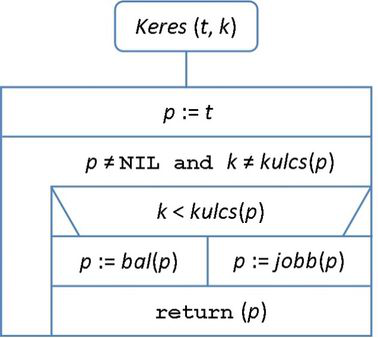
\includegraphics[width=0.3\textwidth]{img/bin_tree_iterative.png}
		\caption{A keresés műveletének iteratív algoritmusa}
	\end{figure}

    \subsubsection*{A legkisebb kulcs keresése}

    \noindent Egy nem üres bináris keresőfában úgy jutunk el a minimális kulcsot tároló csúcshoz, hogy a gyökértől indulva mindig a bal oldali pointeren lépünk tovább. Ha már nem vezet tovább balra út, akkor megtaláltuk a legkisebb kulcsot.
	\begin{figure}[H]
		\centering
        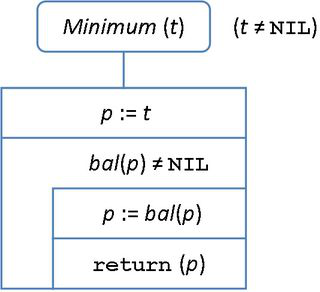
\includegraphics[width=0.25\textwidth]{img/btree_min.png}
		\caption{A minimális kulcs megkeresése}
	\end{figure}

    \subsubsection*{A következő kulcsérték megkeresése}

    \noindent Általában, az adott pontból szülő pointereken megyünk addig, amíg azok – a szülőből nézve – jobb gyerekre mutató pointerek (ez a sorozat lehet üres is). Utána még egy lépést kell tennünk felfelé egy szülő pointeren, amely – ismét a szülő csúcshoz viszonyítva – bal gyerekhez vezet. A bináris fában található maximális kulcsnak nincs rákövetkezője. Ilyenkor a keresés, ezzel összhangban, $NIL$ pointert ad vissza.

	\begin{figure}[H]
		\centering
		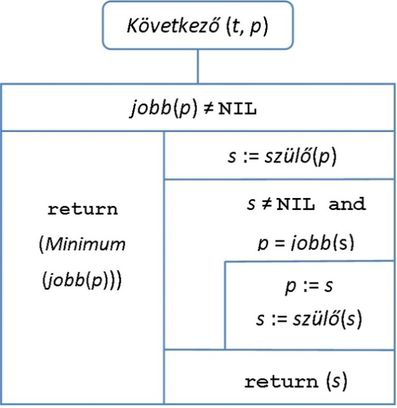
\includegraphics[width=0.30\textwidth]{img/btree_next.png}
		\caption{A nagyság szerint következő kulcs megkeresése}
	\end{figure}

    \subsubsection*{Adott kulcsérték beszúrása}

    \noindent A bináris keresőfába úgy illeszthetünk be – csúcs formájában - egy új kulcsos rekordot, hogy összeállítjuk az új tartalmat egy pontosan olyan szerkezetű rekordban, mint amilyen többi rekord. Az új rekord rendelkezik azzal a három pointer mezővel, amellyel a fában mindegyik fel van szerelve; ezek a bal és a jobb gyerekre, valamint a szülőre mutatnak.

    \noindent Az új rekordra mutató pointert \emph{adjuk oda} a beszúrást végző eljárásnak, amely a már többször látott, balra-jobbra összehasonlító és lépegető stratégiával megkeresi az új kulcs helyét és létrehozza a bináris keresőfa egy új levelét.

    Ha a beillesztendő kulcs különbözik a fa mindegyik kulcsától, akkor sikeres lesz az elhelyezés (ezt az jelzi, hogy az eljárás a p pointer étékét adja vissza), ha viszont megegyezik valamely kulcsértékkel a fában, akkor a sikertelen beszúrást a visszaadott NIL érték jelzi.

	\begin{figure}[H]
		\centering
		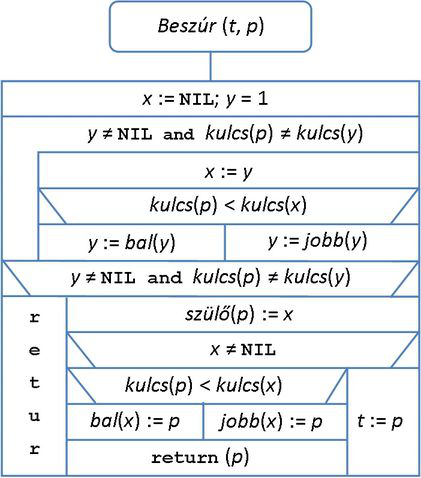
\includegraphics[width=0.40\textwidth]{img/btree_insert.png}
		\caption{Kulcsos rekord beszúrása bináris keresőfába}
	\end{figure}

    \subsubsection*{A keresőfa műveleteinek hatékonysága}

    Ha sorra áttekintjük azt az négy műveletet, amelyet a bináris keresőfákra bevezettünk, akkor azt láthatjuk, hogy mindegyiknek a lényegi részét egy útvonal bejárása adja a fában. Ez az útvonal egy olyan útnak részét képezi, amely a fa gyökerétől valamely levélig terjed. Ennek a befoglaló útvonalnak a hossza attól függ, hogy milyen mélységben található az a levél, amelyben végződik. Minden esetre, a keresőfa magassága felső korlátját képezi a teljes útnak, így a szóban forgó művelet úthosszának is.\\

    A műveletek lépésszáma lényegében megegyezik a fában bejárt útvonal hosszával, amelyhez még hozzá számítunk néhány (konstans számú) lépést.
    Azt mondhatjuk tehát, hogy bináris keresőfa mindegyik $op$ műveletére érvényes az az állítás, hogy lépésszámát nagyságrendben a fa ($h(t)$) magassága felülről korlátozza:
    \begin{center}
        $T_{op}(n) = \mathcal{O}(h(t)) $.
    \end{center}

    A bináris fa a magasságának az alsó korlátját a majdnem teljes fa \emph{összenyomott} állapotában veszi fel, a magasság legnagyobb értékét pedig egy láncszerű fa esetén kapjuk.\\ Érvényes a következő összefüggés:
    \begin{center}
        $\lfloor log_2n \rfloor \leq h(t) \leq n - 1$.\\
    \end{center}

    \noindent A két összefüggés alapján a bináris fa műveleteire a következőket állíthatjuk az
    \begin{itemize}
        \item általános (tetszőleges egyedi) esetben: $T_{op}(n) = \mathcal{O}(n)$, valamint a
        \item legkedvezőbb esetben: $mT_{op}(n) = \mathcal{O}(log n)$, illetve a
        \item legkedvezőtlenebb esetben: $MT_{op}(n) = \mathcal{O}(n)$
    \end{itemize}

	\noindent Az a cél, hogy a bináris keresőfa ne nyúljon meg láncszerűen, erre jó az AVL-fa és a 2-3-fa.
	
	\subsection*{AVL-fa}
	
	Cél: a $t$ bináris keresőfa magasságának $\log_2(n)$ közelében tartása, azaz $h(t) \leq c \cdot \log_2(n)$, ahol $c$ elfogadhatóan kicsi. Az ilyen fát kiegyensúlyozottnak nevezzük. \\
	\textit{AVL}: Adelszon-Velszkij, Landisz 1962-ben alkották meg. \\
	A $t$ bináris keresőfát egyúttal AVL-fának nevezzük $\Longleftrightarrow$ $t$ minden $x$ csúcsára $|h(bal(x))-h(jobb(x))| \leq 1$. \\
	Minden csúcsnak van egy címkéje $+,-,=$ (gyerekek magasságának különbsége). A beszúrás helyétől felfelé ellenőrizzük ezeket, és ha kell, akkor módosítjuk. Ha valahol $++$ vagy $--$ alakul ki, akkor ott elromlik az AVL-tulajdonság, egy vagy több forgatással vagy átkötéssel konstans műveletigénnyel helyre lehet hozni. \\
	Többféle séma is van: $(++,+), (++,-), (++,=)$ és a tükörképeik.
	
	\subsection*{2-3-fa és B-fa}
	
	2-3-fa kis méretben az elmélet számára jó, a B-fa a gyakorlati változat adatbázisban. \\
	$t$ 2-3-fa $\Longleftrightarrow$ minden belső csúcsnak 2 vagy 3 gyereke van, a levelek azonos szinten helyezkednek el, adatrekordok csak a levelekben vannak, belső pontokban kulcsok és mutatók, levelekben a kulcsok balról jobbra nőnek. \\
	Ha 4 gyerek lenne a beszúrás után, akkor csúcsot kell vágni. Ha törlésnél 1 gyerek lenne valahol, akkor csúcsösszevonásokat és gyerekátadást alkalmazunk. \\
	B-fa nagyobb méretű, itt két határ között mozog a gyerekszám: $\lceil\frac{r}{2}\rceil$ és $r$, ahol $50 \leq r \leq 1000$.
	
	\subsection*{Hasítás}
	
	Kulcsos rekordokat tárol.
	\begin{itemize}
		\item \textit{Hasítás láncolással}: a kulcsütközést láncolással oldja fel. Van egy hasítófüggvény: $h: U \to [0..m-1]$, elvárás vele kapcsolatban, hogy gyorsan számolható és egyenletes legyen. $m$-et úgy választjuk meg $n$ nagyságrendjének ismeretében, hogy $\alpha = \frac{n}{m}$ lesz a várható listahossz, ha egyenletes hasítást feltételezünk.\\
		Például kétirányú listát használhatunk a hasításhoz. Műveletek: beszúrás, keresés, törlés. \\
		Gyakorlatban érdemes $m$-et úgy megválasztani, hogy olyan prímszám legyen, ami nem esik 2-hatvány közelébe.
		\item \textit{Hasítás nyitott/nyílt címzéssel}: A kulcsokat lehessen egészként értelmezni, ekkor vannak jó hasítófüggvények. \\
		Próbálkozás általános képlete: $h(k) + h_i(k)$ $(mod$ $M)$, $0 \leq i \leq M-1$. Egész addig alkalmazza, amíg üres helyet nem talál.
		\begin{enumerate}
			\item \textit{Lineáris próba}: $h_i(k) = -i$ $(mod$ $M)$, egyesével balra lépegetve keressük az üres helyet. Hátránya az elsődleges csomósodás, ez jelentős lassulást okoz beszúrásnál és keresésnél.
        	\begin{figure}[H]
    		\centering
	       	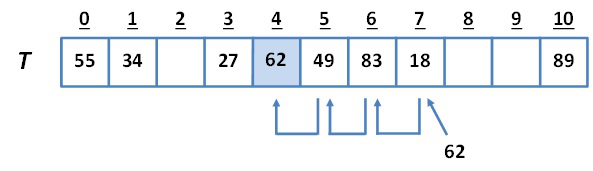
\includegraphics[width=0.45\textwidth]{img/hash_opentest.png}
		      \caption{Nyílt címzés lineáris próbálkozással}
	        \end{figure}
			\item \textit{Négyzetes próba}: $h_i(k) = (-1)^i(\lceil\frac{i}{2}\rceil)^2$ $(mod$ $M)$, a négyzetszámokkal lépegetünk balra-jobbra, ezek az eltolások kiadják $\{0,1,...,M-1\}$-et. Hátrány: másodlagos csomósodás.
        	\begin{figure}[H]
    		\centering
	       	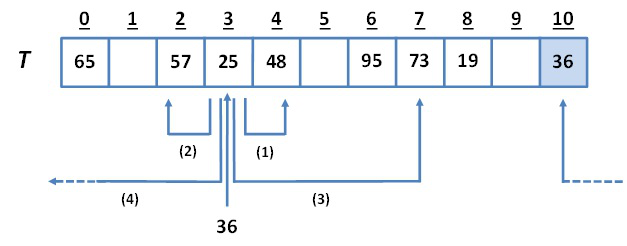
\includegraphics[width=0.45\textwidth]{img/hash_squaretest.png}
		      \caption{Nyílt címzés négyzetes próbálkozással}
	        \end{figure}
			\item \textit{Kettős hash-elés}: $h_i(k) =-ih'(k)$ $(mod$ $M)$, $h'(k)$ a $k$-hoz tartozó egyedi lépésköz, $(h'(k),M)=1$ relatív prímek. Ha az $M$ elég nagy, akkor nincs csomósodás.
        	\begin{figure}[H]
    		\centering
	       	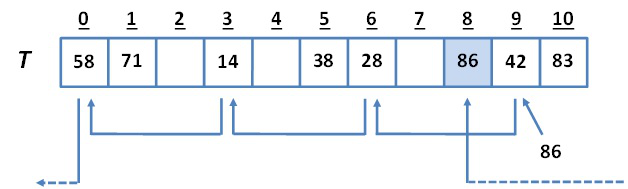
\includegraphics[width=0.45\textwidth]{img/hash_doubletest.png}
		      \caption{Nyílt címzés négyzetes próbálkozással}
	        \end{figure}
		\end{enumerate}
		\item \textit{Hasítófüggvények}: Leggyakoribb: $k$ egész, kongruencia reláció. Általánosan: $h(k) = (ak +b$ $(mod$ $p))$ $(mod$ $M)$, az univerzális hasítás családja. Tapasztalat: $k$ egyenletesen hasít.
	\end{itemize}
	
	\section*{Összehasonlító rendező algoritmusok}

	\subsection*{Buborékrendezés}
	
	A buborékrendezés az egyik legrégebbi ismert rendezés. Lényege az, hogy a maximális elemet cserékkel ,,felbuborékoltatjuk" a tömb végére, és így visszavezetjük a problémát egy 1-gyel rövidebb rendezési feladatra. A buborékoltatás úgy működik, hogy párosával (mintha egy két elem szélességű ablakot léptetnénk) haladunk végig az elemeken és a rossz sorrendben lévő párokat megcseréljük. Ezt az eljárást a \ref{fig:bubblesort_sample}. ábra szemlélteti.
	\begin{figure}[H]
		\centering
		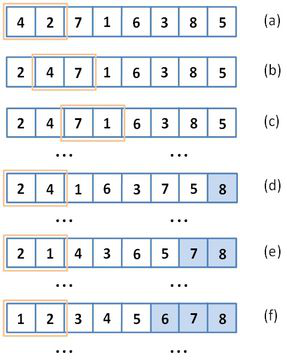
\includegraphics[width=0.3\textwidth]{img/bubblesort_sample.png}
		\caption{A buborékrendezés működése}
        \label{fig:bubblesort_sample}
	\end{figure}

    Belátható, hogy így a legnagyobb elem eljut egészen a tömb végéig. (Ha több maximális elem is van a tömbben, akkor közülük a jobboldali jut el a tömb végére, mert egy egyenlő elempár esetén nem hajtunk végre cserét.) A második felbuborékoltatásnál már a tömb utolsó elemét nem kell figyelembe vennünk, hiszen tudjuk, hogy az jó helyen van.\\

    Indukcióval látható, hogy a k-adik felbuborékoltatáskor az utolsó $k-1$ elem a tömb jobb szélén helyezkedik el, rendezve.\\

    A rendezés algoritmusa a \ref{fig:bubblesort}. ábrán látható. (A működés leírásában saját ciklusszervezést használtunk.)

	\begin{figure}[H]
		\centering
		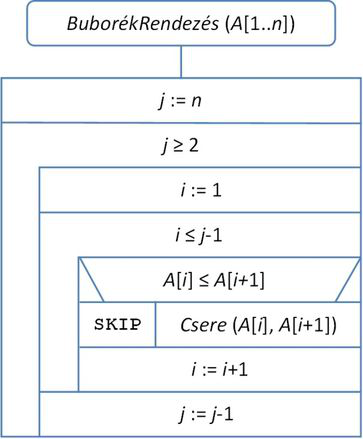
\includegraphics[width=0.3\textwidth]{img/bubblesort.png}
		\caption{A buborékrendezés algoritmusa}
        \label{fig:bubblesort}
	\end{figure}

    \noindent Műveletigény:
    \begin{itemize}
        \item Legrosszabb eset: $\Theta(n^2)$
        \item Átlagos eset: $\Theta(n^2)$
    \end{itemize}
	
	\subsection*{Beszúró rendezés}
	
    A beszúró rendezés sok esetben a leggyorsabb négyzetes rendezés. Működése hasonló ahhoz, mint amikor lapjainkat rendezzük egy kártyajáték során. A rendezés fő lépése az, hogy az asztalon lévő rendezetlen saját pakliból elvesszük a felső lapot és beszúrjuk a kezünkben tartott rendezett lapok közé. Kezdetben a rendezett rész az első felvett lapból áll, majd $n - 1$ beszúrás után lapjainkat már rendezett módon tartjuk a kezünkben.

    A beszúró rendezés még nem említett előnye az, hogy nem csak tömbben tárolt elemek rendezésére alkalmas, hanem a láncolt listákra is könnyen alkalmazható.

    \subsubsection*{Tömbös megvalósítás}

    A tömbben tárolt adatok rendezésére alkalmazott beszúró rendezés működését, egy-egy jellemző lépés megjelenítésével a \ref{fig:insertsort_sample}. ábra szemlélteti.

	\begin{figure}[H]
		\centering
		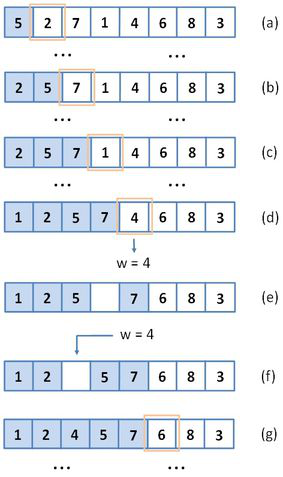
\includegraphics[width=0.3\textwidth]{img/insertsort_sample}
		\caption{A beszúró rendezés működése tömbös megvalósítás esetén}
        \label{fig:insertsort_sample}
	\end{figure}

    Tömbös megvalósítás esetén a rendezett részt a tömb elején tároljuk, a rendezetlent pedig utána. Kezdetben csak a tömb első eleme rendezett. Minden iterációban a következőnek beszúrandó elemet elmentjük egy $w$ változóba, majd az eddig rendezett rész nála nagyobb elemeit jobbra csúsztatjuk egy pozícióval.\\

    A megfelelő számú léptetés után felszabadul a félretett beszúrandó elem számára a megfelelő hely. Ezután a beszúrandó elemet $w$-ből bemásoljuk a megfelelő helyre. A teljes algoritmus a \ref{fig:insertsort}. ábrán látható.

	\begin{figure}[H]
		\centering
		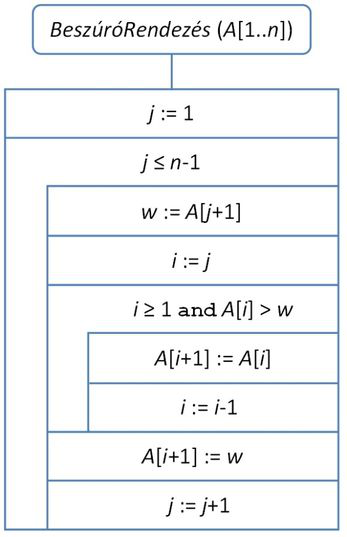
\includegraphics[width=0.3\textwidth]{img/insertionsort.png}
		\caption{A beszúró rendezés algoritmusa tömbös megvalósítás esetén}
        \label{fig:insertsort}
	\end{figure}
	
    Algoritmusunk egy külső és egy belső ciklusból áll. A külső ciklus beszúrásonként lép egyet, míg a belső ciklus a beszúrás közbeni jobbra másolásokért felelős. A külső ciklus addig halad, amíg minden elemet be nem illesztettünk a helyére, a belső pedig addig, amíg meg nem találtuk az aktuálisan beszúrandó elem helyét.\\

    A külső ciklus mindig $n-1$ alkalommal fut le, hiszen ennyi elemet kell beszúrnunk a rendezett részbe, ahhoz hogy az egész tömb rendezve legyen.\\

    \noindent Műveletigény:
    \begin{itemize}
        \item Legrosszabb eset: $\Theta(n^2)$
        \item Átlagos eset: $\Theta(n^2)$
    \end{itemize}

	\subsection*{Versenyrendezés}

    \noindent A versenyrendezés a versenyfa (tournament) adatszerkezetet használja. A versenyfa olyan teljes bináris fa, amelynek a leveleiben helyezkednek el a rendezendő elemek. Szintfolytonosan ábrázoljuk tömbösen. A \ref{fig:tournament_start}. ábrán egy kitöltött levelekkel rendelkező, de a belső pontjaiban még kitöltetlen versenyfát láthatunk.

	\begin{figure}[H]
		\centering
		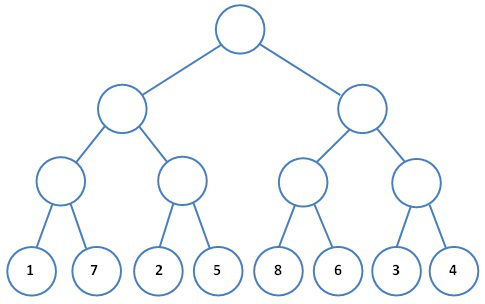
\includegraphics[width=0.4\textwidth]{img/tournament_start.png}
		\caption{Versenyfa, leveleiben a rendezendő számokkal}
        \label{fig:tournament_start}
	\end{figure}	

    \noindent A fa belső pontjait szintenként úgy töltjük ki, ahogyan egy kieséses verseny halad előre: minden belső pontban a gyerekei közül a nagyobbnak az értéke kerül (mint egy mérkőzés nyertese). Végül, a maximum (az abszolút győztes) a fa gyökerébe kerül. A kitöltött versenyfát a \ref{fig:tournament_fill1}. ábra szemlélteti, $n=8$ rendezendő szám esetére.

	\begin{figure}[H]
		\centering
		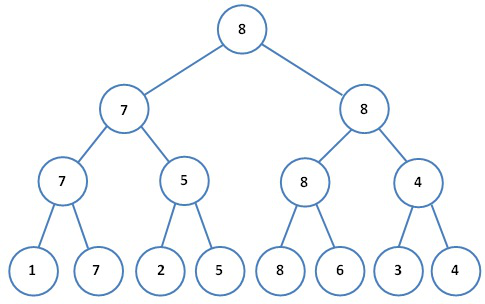
\includegraphics[width=0.4\textwidth]{img/tournament_fill1.png}
		\caption{Kitöltött versenyfa}
        \label{fig:tournament_fill1}
	\end{figure}	

    \noindent A rendezés egy speciális első menetet, majd azután még $(n – 1)$ egyszerűbb iterációs lépést hajt végre. Az első menetben – a versenyfa imént leírt kitöltésével – kiválasztjuk a legnagyobb elemet, amely \emph{felkerül} a fa gyökerébe. Vegyük hozzá ehhez még a legnagyobb elem kiírását is, a rendezés kimenetére. Ezt már a következő \ref{fig:tournament_max}. ábra tünteti fel.

	\begin{figure}[H]
		\centering
		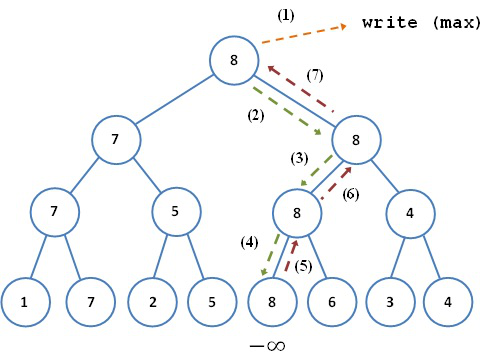
\includegraphics[width=0.4\textwidth]{img/tournament_max.png}
		\caption{Az első "újrajátszás" a győztes ágán}
        \label{fig:tournament_max}
	\end{figure}	

    \noindent A versenyfa kitöltését követően kerül sor $(n – 1)$ egyszerűbb menetre, a következő legnagyobb elem kiválasztására. Példánkban ez $(8 – 1 = 7)$ iterációt jelent, amelyek közül az első kettő lépéseit mutatja be a \ref{fig:tournament_max}. és a \ref{fig:tournament_max2}. ábra.\\

	\begin{figure}[H]
		\centering
		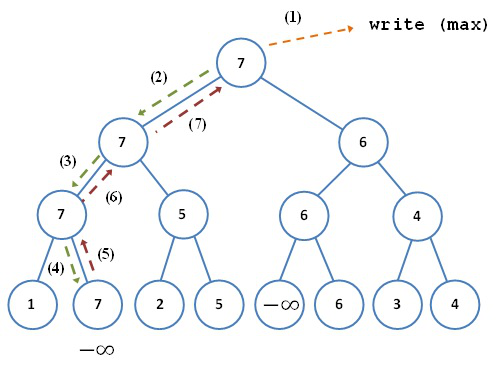
\includegraphics[width=0.4\textwidth]{img/tournament_max2.png}
		\caption{A második "újrajátszás" a következő győztes ágán}
        \label{fig:tournament_max2}
	\end{figure}

    \noindent Miután a gyökérben megjelenő legnagyobb elemet kiírtuk, \emph{lefelé} haladva megkeressük azt a levelet, amelyben eredetileg ez az érték helyet foglal. A levélben található értéket (mínusz végtelen)-re cseréljük, azaz egy abszolút vesztest teszünk a helyére. Utána \emph{felfelé} haladva ezen az ágon \emph{újrajátsszuk a mérkőzéseket}. Ezeket a lépéseket sorszámozott formában láthatjuk a \ref{fig:tournament_max}. ábrán.\\

    \noindent Az újrajátszás eredményét már a következő \ref{fig:tournament_max2}. ábra tünteti fel. A második legnagyobb elem megjelent a gyökérben. Ez által azt is megtudjuk, hogy \emph{ki nyert volna, ha a győztes nem indult volna a versenyen}. Ezen az ábrán bejelöltük a második legnagyobb elem levélszintű helyének a megkeresését és az ezt követő újrajátszás útvonalát.\\

    \noindent Így haladunk tovább, minden menetben a következő legnagyobb elemet megkeresve és kiírva. Mivel az elemeket csökkenő sorrendben vettük ki, az eljárás alkalmas a rendezés megvalósítására.

	\begin{figure}[H]
		\centering
		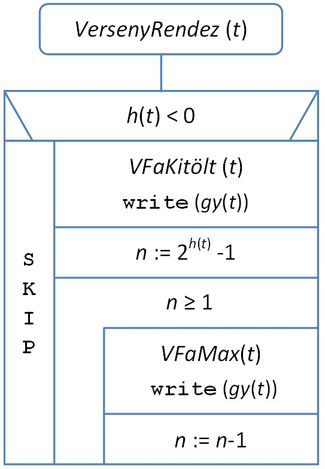
\includegraphics[width=0.32\textwidth]{img/tournamentsort.png}
		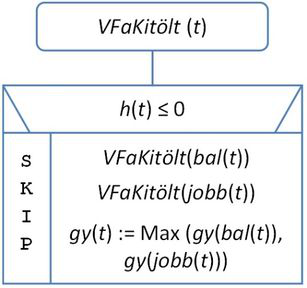
\includegraphics[width=0.32\textwidth]{img/vtree_fill.png}
		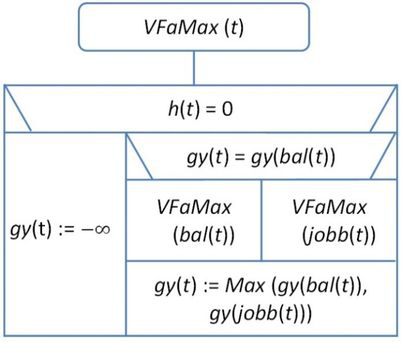
\includegraphics[width=0.32\textwidth]{img/vtree_max.png}
		\caption{Versenyrendezés}
	\end{figure}
	
    \noindent Műveletigény:
    \begin{itemize}
        \item Legrosszabb eset: $\Theta(n \cdot log\ n)$
        \item Átlagos eset: $\Theta(n \cdot log\ n)$
    \end{itemize}

	\subsection*{Kupacrendezés}

    \noindent A kupacrendezés algoritmusa két fő részből áll. Az első részben felépíti az inputból a kupacot (KezdőKupac), a másodikban pedig visszaírja a kimenetbe a kupacból az elemeket. A kupac felépítése az elemek egyenkénti beszúrásával történik az Insert és a MoveUp kupacműveletek segítségével úgy, hogy minden lépésben megmaradjon a kupac-tulajdonság. A beszúrásokat addig folytatja, amíg a bemeneti tömb kiürül. A második lépésben a TakeOut és Süllyeszt műveletekkel kiírja az aktuális gyökérelemet a kimenetbe, a helyére beszúrja a  legszélső levél tartalmát, és rendezi a kupacot. Addig ismétli ezt a lépést, amíg üres kupacot nem kapunk.

    \subsubsection*{Tömbös megvalósítás}

    \noindent Mivel programozásban egyszerűbb a kupac tömbös megvalósításával dolgozni, ezért a rendezést úgy hajtjuk végre, mintha egy szintfolytonos bejárással létrehozott tömbön végeznénk. Ebben a felfogásban első lépésként úgy rendezzük az inputot, hogy végig megyünk a tömbön, megvizsgáljuk az aktuális elem és a leszármazottjai viszonyát, és ahol nem teljesül a kupac tulajdonság, ott a nagyobbikkal megcseréljük (ez felel meg a Süllyeszt műveletnek). Addig folytatjuk a cseréket, amíg egy kupacnak megfeleltethető tömböt kapunk.\\

    \noindent A második szakaszban a gyökérelem, vagyis az éppen aktuális maximum mindig a tömb elején fog elhelyezkedni, míg a jobb alsó elem a tömb még rendezetlen részének végén lesz. A gyökérelem kivétele és a jobb alsó elem beszúrása megfeleltethető a két elem cseréjének,  ami után a tömb rendezetlen részének mérete eggyel csökken. Ha a beszúrt elem kisebb, mint a nagyobbik leszármazottja, akkor átrendezzük a tömböt úgy, hogy ismét megfeleljen a kupac definíciónak.\\

    \noindent Az újrarendezés után ismét az első és a rendezetlen rész utolsó elemének cseréjével folytatódik az algoritmus. A rendezés akkor ér véget, ha a tömb rendezetlen részének mérete 1, vagyis a teljes tömb rendezve van.

    \subsubsection*{Kezdőkupac kialakítása}
	
	\begin{figure}[H]
		\centering
		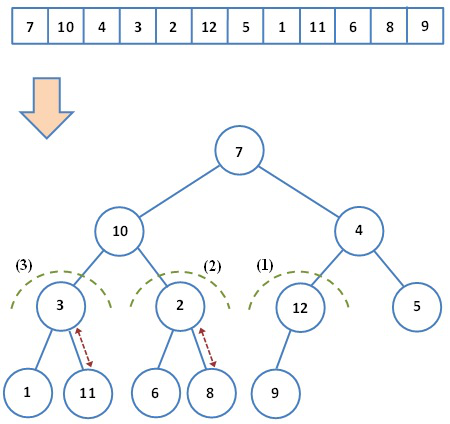
\includegraphics[width=0.4\textwidth]{img/heap_sort_createheap1.png}
		\caption{Kezdőkupac kialakítása (1)}
        \label{fig:heap_sort_createheap1}
	\end{figure}

	\begin{figure}[H]
		\centering
		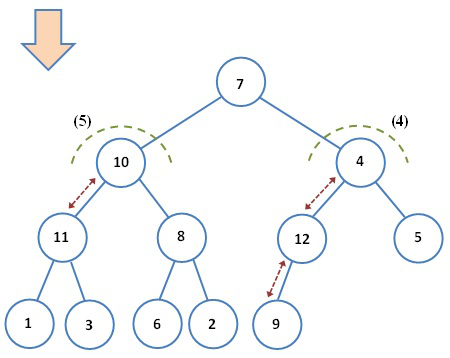
\includegraphics[width=0.4\textwidth]{img/heap_sort_createheap2.png}
		\caption{Kezdőkupac kialakítása (2)}
        \label{fig:heap_sort_createheap2}
	\end{figure}

	\begin{figure}[H]
		\centering
		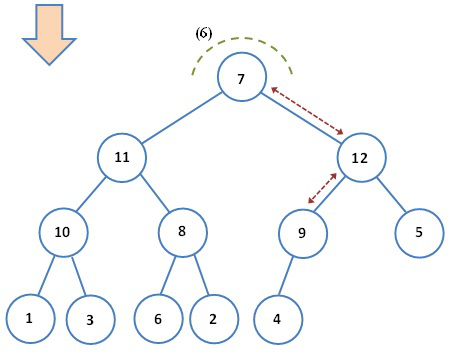
\includegraphics[width=0.4\textwidth]{img/heap_sort_createheap3.png}
		\caption{Kezdőkupac kialakítása (3)}
        \label{fig:heap_sort_createheap3}
	\end{figure}

   	\begin{figure}[H]
		\centering
		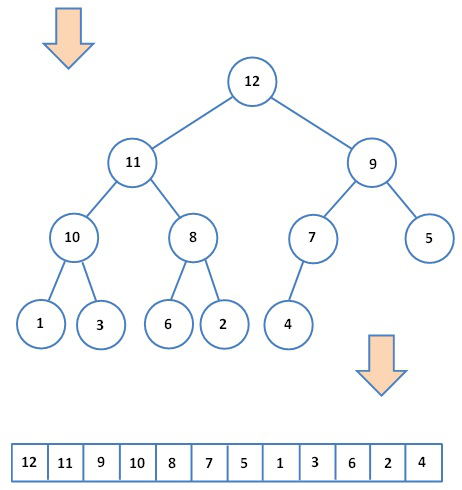
\includegraphics[width=0.4\textwidth]{img/heap_sort_createheap4.png}
		\caption{Kezdőkupac kialakítása (4)}
        \label{fig:heap_sort_createheap4}
	\end{figure}

    \subsubsection*{A következő legnagyobb elem kiválasztása}

   	\begin{figure}[H]
		\centering
		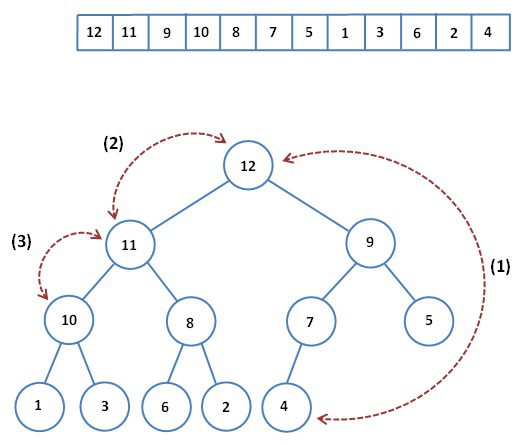
\includegraphics[width=0.4\textwidth]{img/heap_sort_max.png}
		\caption{A maximális elem kiválasztása, elhelyezése és a kupac tulajdonság helyreállítása}
        \label{fig:heap_sort_max}
	\end{figure}

    \subsubsection*{A kupacrendezés teljes eljárása}

   	\begin{figure}[H]
		\centering
		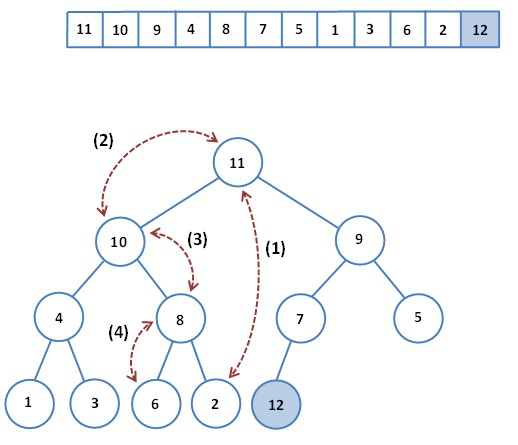
\includegraphics[width=0.4\textwidth]{img/heap_sort1.png}
		\caption{A második legnagyobb elem kiválasztása}
        \label{fig:heap_sort1}
	\end{figure}

   	\begin{figure}[H]
		\centering
		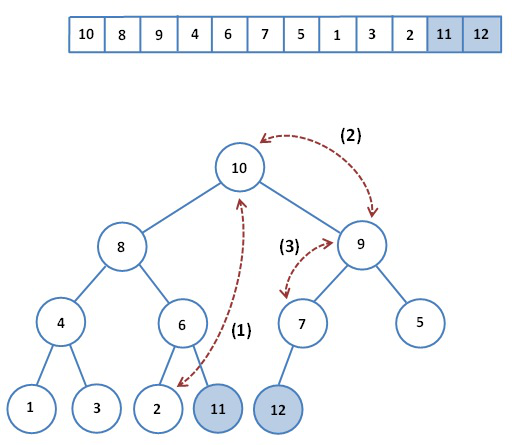
\includegraphics[width=0.4\textwidth]{img/heap_sort2.png}
		\caption{A következő legnagyobb elem kiválasztása}
        \label{fig:heap_sort2}
	\end{figure}

    \begin{center}
        $\cdots$
    \end{center}

   	\begin{figure}[H]
		\centering
		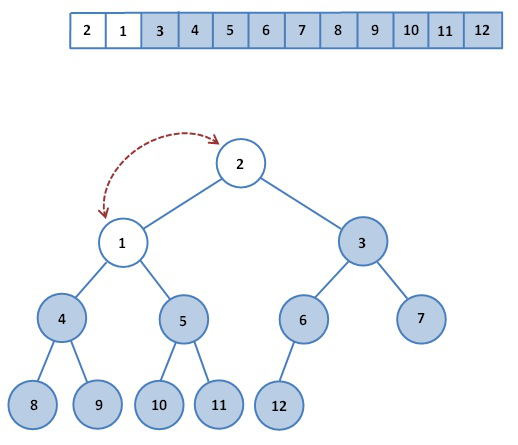
\includegraphics[width=0.4\textwidth]{img/heap_sort3.png}
		\caption{Az utolsó előtti elem kiválasztása}
        \label{fig:heap_sort3}
	\end{figure}

   	\begin{figure}[H]
		\centering
		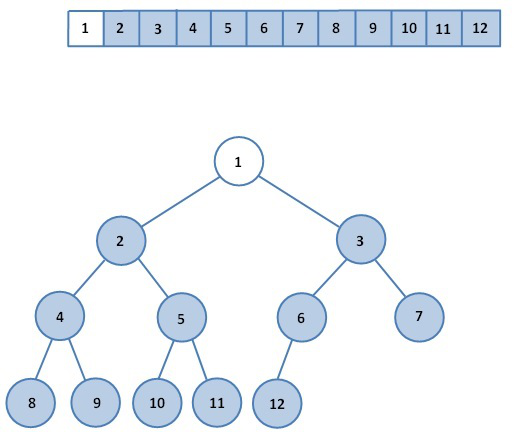
\includegraphics[width=0.4\textwidth]{img/heap_sort4.png}
		\caption{Az utolsó elem kiválasztása, kész kupac}
        \label{fig:heap_sort4}
	\end{figure}

    \subsubsection*{Algoritmusok}

	\begin{figure}[H]
		\centering
		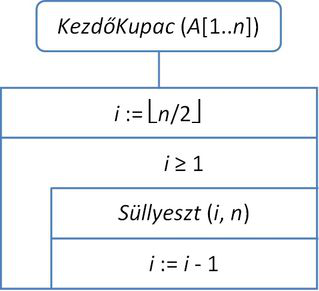
\includegraphics[width=0.32\textwidth]{img/heapsort_start.png}
		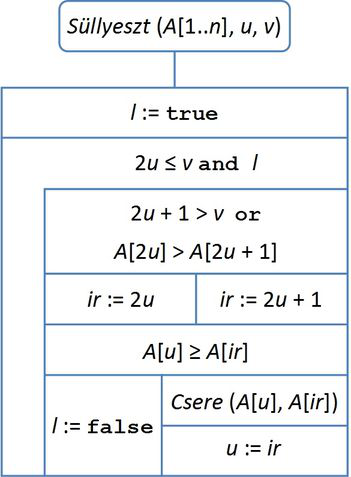
\includegraphics[width=0.32\textwidth]{img/heapsort_pulldown.png}
		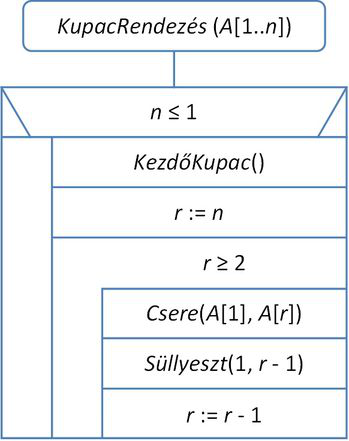
\includegraphics[width=0.32\textwidth]{img/heapsort.png}
		\caption{Kupacrendezés}
	\end{figure}
	
    \noindent A kezdőkupac kialakításánál, és a ciklus közben a süllyesztés módja kicsit különbözik, hiszen az első esetben a változó elem süllyed le a teljes kupacon, a másodikban a gyökér süllyed az aktív kupacon. A képen látható algoritmus mindkét műveletet teljesíti.
	
    \noindent Műveletigény:
    \begin{itemize}
        \item Legrosszabb eset: $\Theta(n \cdot log\ n)$
        \item Átlagos eset: $\Theta(n \cdot log\ n)$
    \end{itemize}

	\subsection*{Gyorsrendezés}
	
    \noindent Az algoritmus Az ,,oszd meg és uralkodj" elvet használja, azaz a problémát kisebb méretű, azonos problémákra bontja, amelyek rekurzívan megoldhatók, majd a megoldásokat egyesíti. Első lépéseként kiválasztunk egy tetszőleges főelemet, ez után a tömböt három részre particionáljuk úgy, hogy a kiválasztott főelemnél kisebb elemeket a főelem elé, a nála nem kisebbeket pedig mögé mozgatjuk. Az így kialakuló három résztömbön - amiket a főelem, a nála kisebb, valamint a nála nagyobb elemek alkotnak - újra futtatjuk a gyorsrendezést. Ez az algoritmus két fő részre bontható, az egyik maga a rekurzív rendezés, a másik pedig a particionálás.

	\begin{figure}[H]
		\centering
        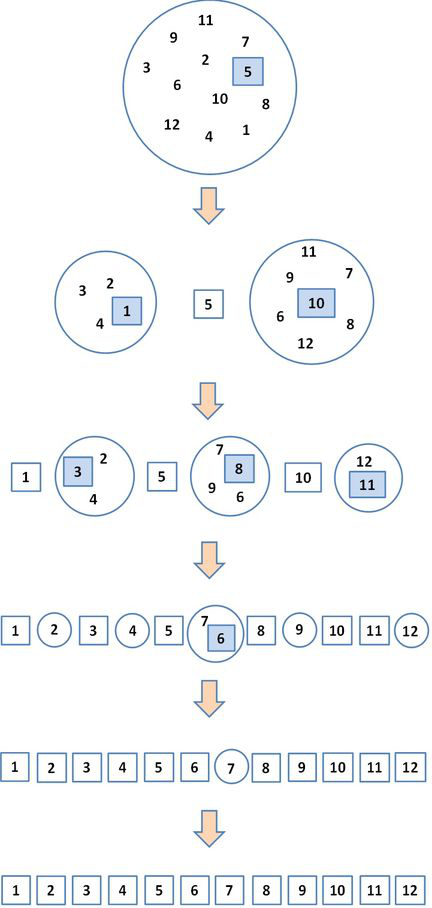
\includegraphics[width=0.4\textwidth]{img/quicksort_sample.png}
		\caption{A gyorsrendezés elve}
	\end{figure}

	\begin{figure}[H]
		\centering
		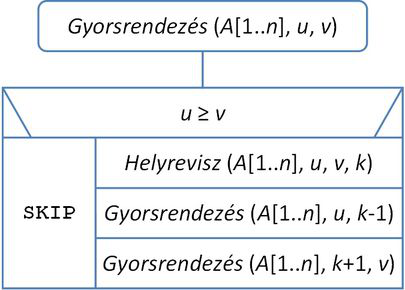
\includegraphics[width=0.35\textwidth]{img/quicksort.png}
		\caption{Az algoritmus megvalósítása tömbre}
	\end{figure}
	\begin{figure}[H]
		\centering
		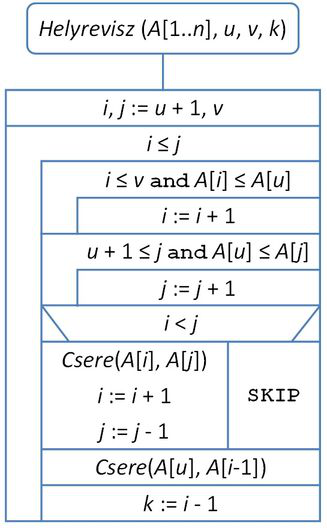
\includegraphics[width=0.3\textwidth]{img/quicksort_move.png}
		\caption{Az egy elemet a helyére vivő eljárás}
	\end{figure}
	
    \noindent Műveletigény:
    \begin{itemize}
        \item Legrosszabb eset: $\Theta(n^2)$
        \item Átlagos eset: $\Theta(n \cdot log\ n)$
    \end{itemize}

	\subsection*{Összefésülő rendezés}
	
    \subsubsection*{Két rendezett sorozat összefésülése}

	\begin{figure}[H]
		\centering
		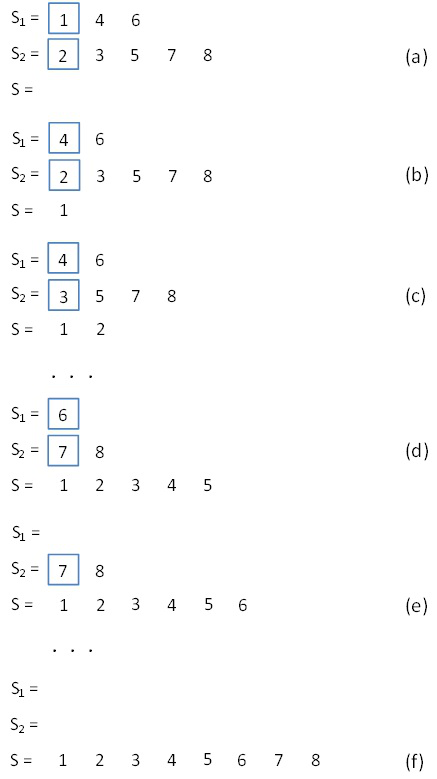
\includegraphics[width=0.35\textwidth]{img/merge_sort_sample.png}
		\caption{Két rendezett sorozat összefésülése}
	\end{figure}

    \noindent Ez a rendezés két már rendezett tömböt fésül össze úgy, hogy a végeredmény is egy rendezett tömb legyen. Az összefésülés folyamata úgy zajlik, hogy mindkét tömb első elemét összehasonlítjuk, és a kisebbet beírjuk a kimeneti tömb első szabad helyére, majd abból  a tömbből, amelyikből ez kikerült, vesszük a következő elemet, és újra elvégezzük az összehasonlítást. Ezt addig folytatjuk, amíg valamelyik kezdeti tömbből el nem fogynak az elemek. Végül másik tömb maradék elemeit is sorban hozzáírjuk az eredményhez, így alakul ki a végleges, rendezett kimeneti tömb. Az algoritmus az összefésülés előtt az inputot rekurzívan kettébontja addig, amíg végül csak rendezett résztömbök lesznek (ez általában az egy elemű résztömb), majd ezeken végzi el az összefésülést. 	Ezt alkalmazhatjuk felülről lefelé (rekurzív) vagy alulról felfelé (iteratív), ez utóbbit szekvenciális fájloknál.\\\\

    \noindent Műveletigény:
    \begin{itemize}
        \item Legrosszabb eset: $\Theta(n \cdot log\ n)$
        \item Átlagos eset: $\Theta(n \cdot log\ n)$
    \end{itemize}

    \subsubsection*{Az összefésülő rendezés rekurzív algoritmusa}

	\begin{figure}[H]
		\centering
		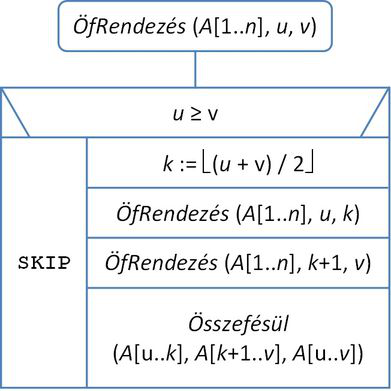
\includegraphics[width=0.4\textwidth]{img/mergesort_alg1.png}
		\caption{Összefésülő rendezés}
	\end{figure}
	
	\section*{Az összehasonlításos rendezések műveletigényének alsó korlátjai}
	
	\subsection*{Műveletigény}
	
    Kijelöljük a domináns műveleteket, és az $n$ inputméret függvényében hányszor hajtódnak végre, ezt nézzük. Jelölés általánosan $T(n)$, de lehet konkrétan is, pl $Cs(n)$ [csere]. $mT(n)$ a minimális műveletigény, $MT(n)$ a maximális és $AT(n)$ az átlagos.	
	\begin{itemize}
		\item[$\Theta$]: nagyságrendileg azonos, két konstans közé beszorítható
		\item[$\mathcal{O}$]: nagyságrendi felső becslés, $o$: nincs megengedve az egyenlőség
		\item[$\Omega$]: nagyságrendi alsó becslés, $\omega$: nincs megengedve az egyenlőség
	\end{itemize}
	
	\begin{figure}[H]
		\centering
        \includegraphics[width=0.4\textwidth]{img/functionsrelations.png}
		\caption{A függvényosztályok egymáshoz való viszonya}
	\end{figure}

    \noindent Aszimptotikus (nagyságrendi) alsó korlátot akarunk adni az összehasonlításokat használó rendező eljárások lépésszámára. Azt akarjuk belátni, hogy egy $n$ méretű input rendezése nagyságrendben legalább $n log n$ összehasonlítást igényel. Ez igaz minden eddig és még nem létező összehasonlításos rendező algoritmusra.

    \subsubsection*{Döntési fa}

    \noindent A döntési fa elkészíthető minden algoritmushoz és annak adott $n$ méretű összes bemenő adatához, feltéve, hogy ezek az adatok felsorolhatók és számuk meghatározható. A rendező eljárásokra ez teljesül, hiszen bemenő adatoknak tekinthetjük az $1,\ 2, \ldots,\ n$ számok permutációit, amelyek $n!$ száma közismert.\\

    \noindent A döntési fa belső pontjaiban tartalmazza az algoritmus által feltett összes igen/nem kimenetelű kérdést, minden lehetséges n méretű bemenő adatra. (Az algoritmus ciklusai az adott n méretű bemenetre történő végrehajtás során egymás utáni lépések szekvenciájává egyenesednek ki, így iteratív vezérlési szerkezetet nem kell megjelenítenünk a fában.) Az esetleges értékadásokat sem helyezzük el a döntési fában. A kérdésekre adott válaszok információtartalmát – az értékadások adattranszformáló hatásának figyelembevételével – minden bemenő adat útvonalán végig haladva fában összegyűjtjük, és a levelekbe írjuk. A döntési fában a levelek tartalma a megoldást fogalmazza meg az egyes inputokra.\\

    \noindent A \ref{fig:decisiontree_sample}. ábrán látható $t_{R}(3)$ döntési fa egy olyan algoritmus működését szemlélteti, amelyet speciálisan három elem rendezésére terveztünk. Az R eljárás az $s1,\ s2,\ s3$ elemek összehasonlítását végzi minden lehetséges input sorrendre. A kérdésekre adott válaszokból meghatározható az elemek nagyság szerint rendezett sorrendje. Ehhez kettő vagy három kérdés szükséges. (Ebben a kis eljárásban értékadások nem szerepelnek.)

	\begin{figure}[H]
		\centering
        \includegraphics[width=0.6\textwidth]{img/decisiontree_sample.png}
		\caption{Az R rendező algoritmus $t_{R}(3)$ döntési fája 3 elemű sorozatokra}
        \label{fig:decisiontree_sample}
	\end{figure}
\newpage
    \noindent \textbf{Lemma}: Bármely $R$ összehasonlító rendező eljárás $t_{R}(n)$ döntési fájának $h(t_{R}(n))$ magassága és az $n$ elemszám között fennáll a következő összefüggés:
    \[
        h(t_{R}(n)) \geq log_{2}n
    \]

	\subsubsection*{Alsó korlát az összehasonlítások számára a legkedvezőtlenebb esetben}
	
    \noindent \textbf{T:} Bármely $R$ összehasonlításos rendező eljárás a legkedvezőtlenebb bemenő adata rendezése során nagyságrendben legalább ($n\ \log\ n$) összehasonlítást végez, azaz
    \[
        \text{MÖ}_{R}(n) = \Omega(n\ \log\ n)
    \]

	\subsubsection*{Alsó korlát az összehasonlítások számára átlagos esetben}

    \noindent \textbf{Lemma:} Az azonos számú levelet tartalmazó tökéletes fák közül levélmagasság összeg azokra a legkisebb, amelyek egyben majdnem teljes bináris fák.\\

    \noindent \textbf{T:} Bármely $R$ összehasonlítás alapú rendező eljárás átlagosan nagyságrendben legalább $n\ log\ n$ összehasonlítást végez az összes lehetséges bemenő sorozat rendezése során:
    \[
        \text{AÖ}_{R}(n) = \Omega(n\ \log\ n)
    \]
	
\end{document} 